\documentclass{article}
\usepackage{geometry}
\usepackage{graphicx}
\usepackage{booktabs}
\usepackage{float}
\usepackage{array}
\usepackage{hyperref}
\usepackage[super,sort&compress]{cite}
\usepackage{listings}
\usepackage{xcolor}

\hypersetup{
    colorlinks=true,
    linkcolor=black,
    citecolor=black,
    urlcolor=blue
}

\lstset{
  language=C,
  basicstyle=\ttfamily\small,
  keywordstyle=\color{blue},
  stringstyle=\color{red},
  commentstyle=\color{gray},
  numbers=left,
  numberstyle=\tiny\color{gray},
  stepnumber=1,
  numbersep=5pt,
  frame=single,
  breaklines=true,
  showstringspaces=false,
  tabsize=2,
  backgroundcolor=\color{gray!10}
}

\newcolumntype{C}{>{\centering\arraybackslash}c}
\title{COMPILER}
\author{Ioannis Michalainas}
\date{March-June 2025}

\begin{document}

\maketitle
\begin{center}
  \textbf{Repository:} \\
  \href{https://github.com/ioannisam/compiler}{github.com/ioannisam/COMPILER}
\end{center}
\bigskip
\begin{abstract}
    This project presents the design and implementation of a compiler for a simple C-style programming language, developed as part of the Programming Languages and Compilers course under Professor \textit{Panagiotis Katsaros}. This project serves as an educational tool.
\end{abstract}

{\small
\tableofcontents
}
\clearpage

\newgeometry{top=1.5cm, bottom=1.5cm, right=1.5cm, left=1.5cm}
\section{Project Structure}
    \subsection{Directory Layout} 
    This project is organized for modularity and clarity. 

    \subsubsection*{main branch}
    The root directory (\texttt{./}) contains general files such as \texttt{README.md}, \texttt{LICENSE}, \texttt{TODO} and the build script \texttt{utils.sh}. Source code is placed under \texttt{src/}, with further separation into \texttt{lexer/} for lexical analysis, \texttt{parser/} for parsing and AST logic and \texttt{codegen/} for code generation, symbol table management and helpers. Header files are located in the \texttt{include/} directory, mirroring the source structure.
    
    During the build process, the \texttt{bin/} directory is created to store the compiler binary, while \texttt{build/} holds generated assembly and compiled binaries. The \texttt{test/} directory contains test cases, divided into \texttt{scripted/} (programs without a \texttt{main} function) and \texttt{structured/} (programs with a \texttt{main} function and additional functions). Documentation is maintained in the \texttt{docs/} directory, which also includes assets such as diagrams.

    \subsubsection*{MIXAL branch}
    The MIXAL branch has identical file structure, but instead of assembly x86, MIXAL code is generated. To compile said code mdk is used through a docker image for compatibility\cite{GNU MDK}.
    
    \begin{figure} [h]
        \centering
        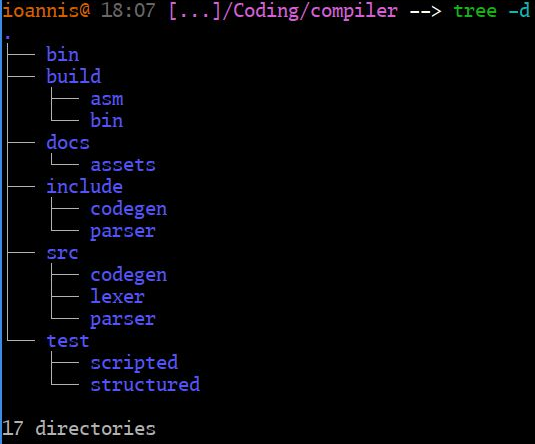
\includegraphics[width=0.75\linewidth]{assets/file-structure.png}
        \caption{File Structure}
        \label{fig:enter-label}
    \end{figure}
    
    \newpage
    \subsection{Build and Utilities} 
    The build process is managed by the \texttt{utils.sh} bash script, which provides a unified interface for generating, compiling, assembling, linking and testing the compiler. The script supports several commands:

    \begin{itemize}
        \item \texttt{generate} invokes Bison and Flex to produce the parser and lexer source files.
        \item \texttt{compile} builds the compiler executable, placing it in the \texttt{bin/} directory.
        \item \texttt{run} executes the compiler on a given input file, generating assembly code in \texttt{build/asm/}.
        \item \texttt{assemble} uses NASM to assemble the generated assembly into an object file.
        \item \texttt{link} produces the final binary using the system linker.
        \item \texttt{binary} runs the compiled program.
        \item \texttt{build} runs the full pipeline: generation, compilation, code generation, assembly, and linking.
        \item \texttt{example} demonstrates the pipeline using a predefined test case.
        \item \texttt{test} automatically runs all test cases in the \texttt{test/} directory, reporting results for each.
        \item \texttt{clean} removes all generated files and build artifacts.
        \item \texttt{help} displays usage information.
    \end{itemize}

    For the MIXAL branch, the build script provides the same functionality but uses different tools, such as \texttt{docker} for system compatibility, \texttt{mixasm} instead of NASM for assembly and \texttt{mixvm} to run the generated programs.
    
    \begin{figure} [h]
        \centering
        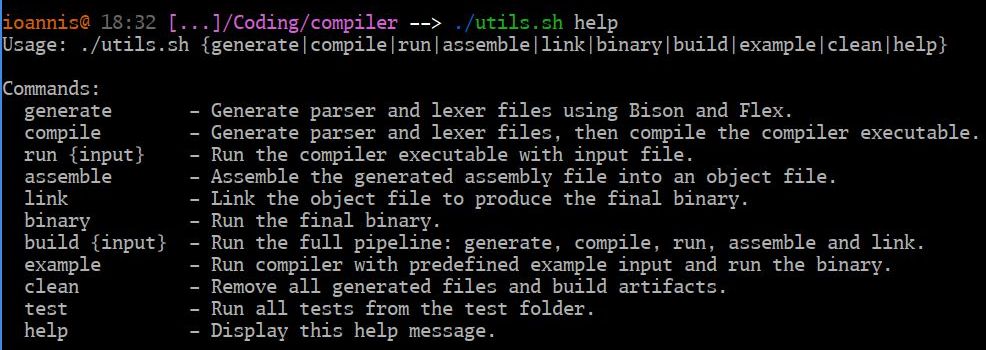
\includegraphics[width=1\linewidth]{assets/utils.png}
        \caption{Utilities}
        \label{fig:enter-label}
    \end{figure}
    
\section{Lexical Analysis}
    \subsection{Lexer Implementation (\texttt{lang.l})} 
    The lexer is implemented using Flex. It recognizes keywords, identifiers, literals, operators and delimiters. Whitespace and comments are ignored. Each token is returned to the parser with its semantic value, such as integer values for numbers or string pointers for identifiers and string literals.
    
    \subsection{Token Definitions} 
    Tokens include keywords (\texttt{int}, \texttt{main}, \texttt{if}, \texttt{else}, etc.), operators (arithmetic, logical, bitwise), delimiters (parentheses, braces, semicolons, commas), literals (numbers, strings) and identifiers. Each token is associated with a unique value for the parser to distinguish during syntax analysis.

\section{Syntax Analysis}

    \subsection{Parser Implementation (\texttt{parser.y})} 
    The parser is written in Bison and defines the grammar for the language. It supports both structured (function-based) and scripted (block-based) modes. The parser constructs an abstract syntax tree (AST) representing the program structure, including functions, statements, expressions and control flow constructs.
    
    \subsection{AST Representation (\texttt{ast.c})} 
    The AST is composed of nodes for each language construct, such as declarations, assignments, function calls, control flow and expressions. Each node type is represented by a C struct, with fields for child nodes and relevant data. Helper functions are provided for constructing and manipulating AST nodes.
    
    \subsection{Error Handling} 
    Syntax errors are reported with line numbers and context using the \texttt{yyerror} function. The parser attempts to recover from errors where possible, allowing multiple errors to be reported in a single run. Accurate newline tracking is essential for providing precise line number information in error messages..

\section{Semantic Analysis}
    \subsection{Symbol Table Management (\texttt{symbol.c})} 
    A symbol table is maintained to track declared variables and function parameters. Each symbol stores its name, type and a unique label for code generation. The symbol table is populated during AST traversal before code generation, ensuring all variables are declared and accessible.

    \subsection{Semantic Error Reporting} 
    Semantic errors, such as undeclared variables or redefinitions, are detected during symbol table operations. Errors are reported with descriptive messages and halt compilation if encountered.

\section{Code Generation}
    \subsection{Assembly x86 (\texttt{codegen/})} 
    The code generator traverses the AST and emits x86-64 assembly code. The output is divided into \texttt{.data}, \texttt{.bss} and \texttt{.text} sections. String literals for print statements are stored in the data section, while variables are allocated in the BSS section. The text section contains the program logic, including function prologues, arithmetic operations, control flow and system calls for I/O and program exit. An \texttt{itoa} routine is included for integer-to-string conversion during print operations. The entry point is either the \texttt{main} function or a top-level block, depending on the program mode.

    \subsection{MIXAL (\texttt{codegen/})}

    The MIXAL backend emits assembly code for the MIX architecture, mirroring the structure of the x86 backend but with MIX-specific conventions\cite{The Art of Computer Programming}. String literals for print statements are defined using the \texttt{ALF} directive and split into 5-character blocks. Variables and temporaries are declared at the end of the program with the \texttt{CON} directive, rather than in a separate BSS section\cite{Computer Organization and Assembly Language Programming}.
    
    Program logic is organized under a \texttt{START} label, which either jumps to the \texttt{main} function or executes a top-level block, depending on the program mode. Arithmetic, logic, and control flow are implemented using MIXAL instructions (\texttt{ADD}, \texttt{SUB}, \texttt{MUL}, \texttt{DIV}, etc.), with conditional jumps and unique labels for flow control. Function calls and returns use explicit jump instructions and temporary storage for return addresses.

    It is important to note that MIX is an imaginary computer and therefore the capabilities and support of its corresponding assembly language, MIXAL, are limited. As a result, the MIXAL version supports far fewer features than the x86 assembly version of this compiler.

\newpage
\section{Testing and Validation}
    \subsection{Scripted Tests} 
    Scripted tests consist of code blocks without explicit function definitions. These are parsed and executed as the main program body. Test cases validate language features such as variable declarations, assignments, arithmetic and print statements.
    
    \subsection*{Test Cases}
    \subsubsection*{syntax-errros.txt}
        \begin{lstlisting}
{   
    // deliberate errors
    print 1 + 2;
    print (3 * 4;
    if (5 < 6) {
        x = 7;
        y = 8 +;
    }
}
        \end{lstlisting}
        
        \begin{figure} [h]
            \centering
            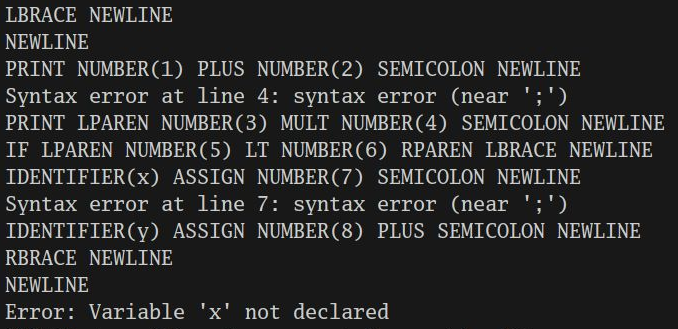
\includegraphics[width=0.35\linewidth]{assets/results/errors.png}
            \caption{Error Output}
            \label{fig:enter-label}
        \end{figure}

    \subsubsection*{precedence.txt}
    \begin{lstlisting}
{
    // output should be -2
    print "-5 + 3*(2-1) - 5%2 + 3/2 = ";
    print -5 + 3*(2-1) - 5%2 + 3/2;
}
    \end{lstlisting}
    \textbf{OUTPUT:} -2

    \subsubsection*{break-nested.txt}
        \begin{lstlisting}
{
    int x = 0;
    while (x<2) {
    
        while (1) {
            print "In the nest...";
            break;
            print "...after the break";
        }
        x = x+1;
    } // should print the first message twice
}
    \end{lstlisting}
    \textbf{OUTPUT:} In the nest... \\ \hspace*{5.7em}In the nest...

    \newpage
    \subsection{Structured Tests} 
    Structured tests use explicit function definitions, including a \texttt{main} function as the entry point. These tests cover function calls, parameter passing, return values, and control flow constructs. Both types of tests ensure correctness of parsing, semantic analysis, and code generation.

    \subsection*{Test Cases}
    \subsubsection*{main.txt}
    
    \begin{lstlisting}
int main() {
    int a = 4;
    print a;
    
    int b;
    b = a+10;
    return b;
}
    \end{lstlisting}
    \textbf{OUTPUT:} 4 [ble: exit 14]
    
    \subsubsection*{digits.txt}
    \begin{lstlisting}
int digits(int num) {

    int dig = 0;
    while (num > 0) {
        dig = dig + 1;
        num = num/10;
    }

    return dig;
}

int main() {
    print digits(42);
    return 0;
}
    \end{lstlisting}
    \begin{figure} [h]
        \centering
        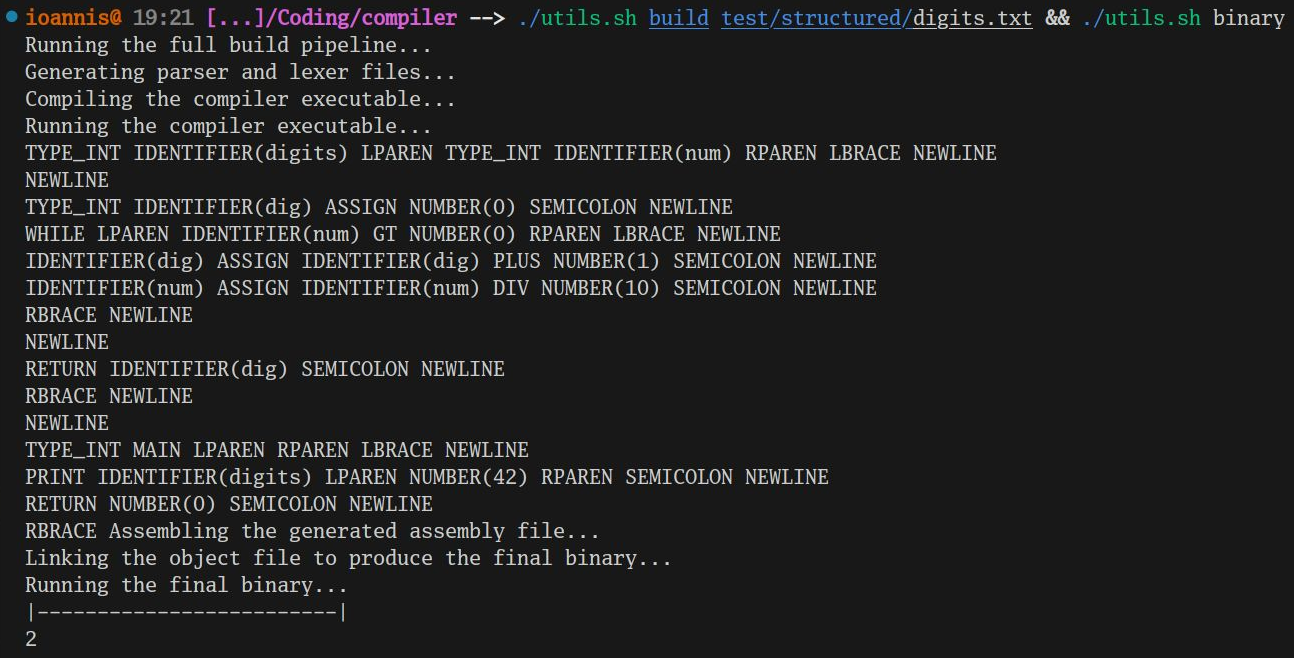
\includegraphics[width=0.75\linewidth]{assets/results/digits.png}
        \caption{Digits Output}
        \label{fig:enter-label}
    \end{figure}

    \newpage
    \subsubsection*{calculator.txt}
    \begin{lstlisting}
int add(int a, int b) {
    return a+b;
}

int sub(int a, int b) {
    return a-b;
}

int mult(int a, int b) {
    return a*b;
}

int div(int a, int b) {
    if (b == 0) {
        // handle undefined
        return 0; 
    } else {
        return a/b;
    }
}

int main() {

    int a = 4;
    print "a is ";
    print a;
    int b = 2;
    print "b is ";
    print b;

    print "a+b = ";
    print add(a,b);
    print "a-b =";
    print sub(a,b);
    print "a*b =";
    print mult(a,b);
    print "a/b =";
    print div(a,b);

    return 0;
}
    \end{lstlisting}
    
    \begin{figure} [h]
        \centering
        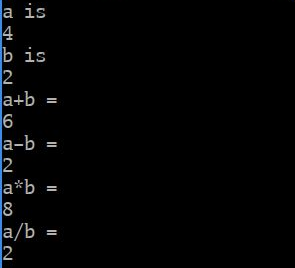
\includegraphics[width=0.35\linewidth]{assets/results/calculator.png}
        \caption{Calculator Output}
        \label{fig:enter-label}
    \end{figure}

\appendix
\section{Future Work and TODO}
Future work includes extending the language with additional data types, keywords, instructions and implementing further optimizations. Increased testing and thorough code review will also be necessary to ensure robustness and to address any remaining corner cases or errors.

\section{Tools and Frameworks}
The following tools and frameworks were used:
\begin{itemize}
  \item Bison
  \item Flex
  \item GCC
  \item NASM
  \item LD
  \item MDK
\end{itemize}

\begin{thebibliography}{9}
    \bibitem[\href{https://data-https://www.gnu.org/software/mdk/}{1}]{GNU MDK}
    GNU MDK
    \bibitem[\href{http://www.jklp.org/profession/books/mix/index.html}{2}]{Computer Organization and Assembly Language Programming}
        Computer Organization and Assembly Language Programming
    \bibitem[\href{https://www-cs-faculty.stanford.edu/~knuth/taocp.html}{3}]{The Art of Computer Programming}
    Donald E. Knuth, \textit{The Art of Computer Programming}, Addison-Wesley.
\end{thebibliography}
\vspace{1em}
\noindent\textbf{Teacher's Lab Notes:} Materials and guidance provided by \textit{Panagiotis Katsaros} during the course Programming Languages and Compilers. Lab documentation was used as a reference for this project.

\end{document}